	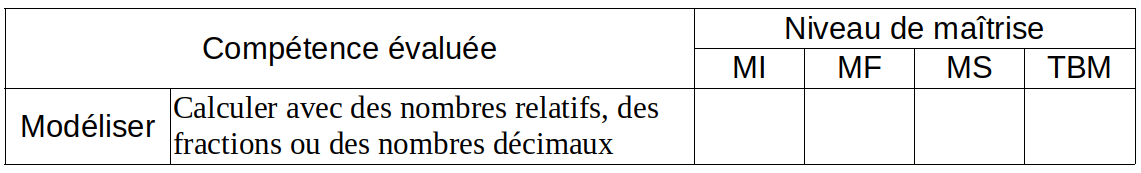
\includegraphics[scale=0.4]{competences}

\section{Calculer}
Calculer les expressions suivantes en détaillant tous les calculs:
\begin{questions}
	
	
	\question[3]  $A = 44 - 37 + 28 - 15$
	
	\fillwithdottedlines{6cm}
	{\LARGE \begin{solution}
		\begin{eqnarray*}
		A &=& 44 - 37 + 28 - 15 \\
		A &=& 7 + 28 - 15 \\
		A &=& 35 -15 \\
		A &=& 20
		\end{eqnarray*}
	\end{solution}}
	
	
	
\question[3]  $B = (7 - 5) \times (8 + 2)$
	
	\fillwithdottedlines{6cm}
	{\LARGE \begin{solution}
		\begin{eqnarray*}
		B &=& (7 - 5) \times (8 + 2)\\
		B &=& 2 \times 10 \\			
		B &=& 20
		\end{eqnarray*}
	\end{solution}}
	
	\newpage
	 \question[4]  $C = 44 - (37 + 28) - 15$
	
	\fillwithdottedlines{5cm}
	{\LARGE \begin{solution}
		\begin{eqnarray*}
		C &=&  44 - (37 + 28) - 15\\
		C &=&  44 - 65 - 15\\
		C &=& (- 11) - 15\\
		C &=& - 26
		\end{eqnarray*}
	\end{solution}
	}
	
	
	\question[4]  $D = (50 + (13 - 1) \times 2) + 6$
	
	\fillwithdottedlines{5cm}
	{\LARGE \begin{solution}
		\begin{eqnarray*}
		D &=&  (50 + (13 - 1) \times 2) + 6\\
		D &=&  (50 + 12 \times 2) + 6\\
		D &=& (50 + 24) + 6\\
		D &=& 74 + 6 \\
		D &=& 82 
		\end{eqnarray*}
	\end{solution}}
	
	
%	{\LARGE \question[2]  $E = (19 + 7 \times 2) - 4$}
%	
%	%\fillwithdottedlines{6cm}
%	{\LARGE \begin{solution}
%		\begin{eqnarray*}
%		E &=&  (19 + 7 \times 2) - 4\\
%		E &=&  (19 + 14) - 4\\
%		E &=& 33 - 4 \\
%		E &=& 29 
%		\end{eqnarray*}
%	\end{solution}}
\end{questions}


\section{Traduire}
Traduire les expressions suivantes par une phrase, sans faire les calculs.
\begin{questions}
	
	\question[3]  $E = 63 + 45 \times 7$
	\fillwithdottedlines{3cm}
	
	
	\question[3]  $F = (73 - 5) \times (24 \div 9)$
	\fillwithdottedlines{3cm}
\end{questions}